\documentclass[aspectratio=169, usenames,dvipsnames, 14pt]{beamer}
\usepackage[utf8]{inputenc}
\usepackage[utf8]{inputenc}
\usepackage{multirow}
\usepackage{gensymb}
\usepackage[absolute,overlay]{textpos}
\usepackage[export]{adjustbox}
\usepackage[absolute,overlay]{textpos}  % Absolute placement of text in frame
\usepackage{xcolor}
\usepackage{animate}

% \usepackage[dvipsnames]{xcolor} % Testing for color of slide 11
\usepackage{listings}           % For source code fonts
\usepackage{tikz}               % For absolute image placement and shapes
\usepackage{Formatting/python_formatting}   % User defined formatting file for source codes

% \usepackage{Formatting/grid_overlay}        % Grid overlay for accurate placement of images

\usepackage{fancyvrb}
\usetikzlibrary{calc}           % For absolute image placement
\usetikzlibrary{decorations.pathreplacing}      % For curly braces

\usetikzlibrary{arrows, positioning, shapes.geometric, quotes, angles}

\mode<presentation>
\usetheme{Rochester}


\newenvironment<>{commandlineblock}[1]{%
  \begin{actionenv}#2%
      \def\insertblocktitle{#1}%
      \par%
      \mode<presentation>{%
        \setbeamercolor{block title}{fg=black,bg=gray!50}
       \setbeamercolor{block body}{fg=white,bg=black!100}
     }%
      \usebeamertemplate{block begin}}
    {\par\usebeamertemplate{block end}\end{actionenv}}


\title{\textbf{Optimizing Trajectories with Dymos}}
\author{Rob Falck}
\date{October 29, 2019}

\begin{document}

%---------------------------------------------------------------------
\begin{frame}
    
    \maketitle

    \tikz[remember picture, overlay] \node[anchor=center] at ($(current page.center)-(5,2)$) {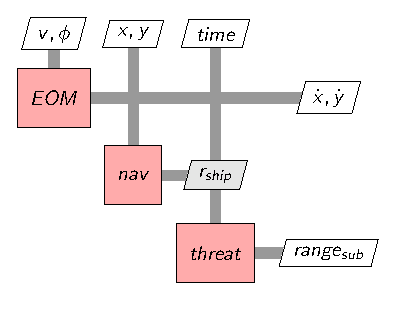
\includegraphics[scale=0.35]{images/donner_sub/donner_sub_ode_xdsm}};

    \tikz[remember picture, overlay] \node[anchor=center] at ($(current page.center)-(-5,2)$) {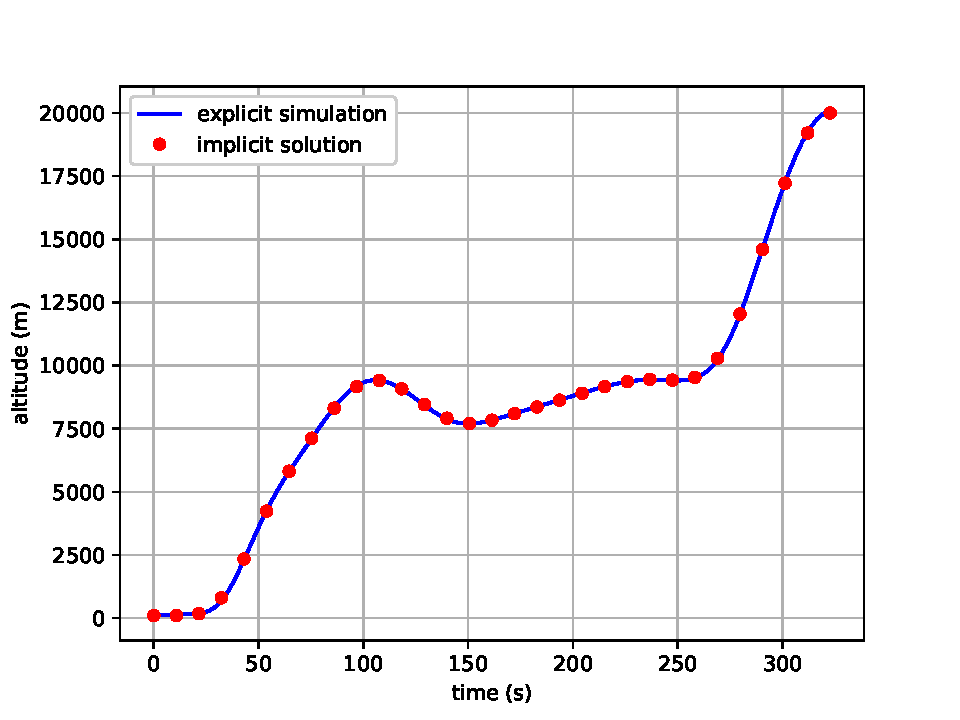
\includegraphics[scale=0.25]{images/min_time_climb_solution.pdf}};

    \tikz[remember picture, overlay] \node[anchor=center] at ($(current page.center)-(0,-3.1)$) {
\includegraphics[scale=0.24]{images/omdao.png}};

%    \tikz[remember picture, overlay] \node[anchor=center] at ($(current page.center)-(-5,3.4)$) {
\includegraphics[scale=0.21]{images/michiganlogo.png}};

\end{frame}
%---------------------------------------------------------------------

\begin{frame}{Dymos is an open-source library for modeling dynamic systems within OpenMDAO}
    \begin{itemize}
        \item Support for multiple optimal control techniques
        \vspace{0.25cm}
        \item Doesn't impose the trajectory optimization as the ``top-level'' problem
        \vspace{0.25cm}
        	\begin{itemize}
        	  \item Treats the trajectory as on component of a larger system
    		  \vspace{0.25cm}
		      \item Design a system to satisfy multiple design reference trajectories
		    \end{itemize}
        \vspace{0.25cm}
		\item Find the best system to fly a trajectory, and the best trajectory that can be flown by the system
    \end{itemize}
\end{frame}

\begin{frame}{Dymos leverages the strengths of OpenMDAO}
    \begin{itemize}
        \item Analytic derivatives and automatic detection of sparsity patterns
        \vspace{0.25cm}
        	\begin{itemize}
        	  \item Adjoint differentiation tends to be faster for shooting methods
              \vspace{0.25cm}
        	  \item Pseudospectral methods tend to be faster in forward mode
              \vspace{0.25cm}
	  		  \item Bidirectional sparsity for problems which would ``break'' pure forward or reverse sparsity
	        \end{itemize}
        \vspace{0.25cm}
		\item Parallelization of expensive models via MPI
        \vspace{0.25cm}
        \item Access to OpenMDAO solvers within the ODE
    \end{itemize}
\end{frame}

\begin{frame}{Dymos Numerical Methods}
    \begin{itemize}
	  	\item Pseudospectral methods
		\vspace{0.25cm}
		    \begin{itemize}
		      \item High-Order Gauss-Lobatto (OTIS)
    		  \vspace{0.25cm}
		      \item Radau Pseudospectral Method (GPOPS, DIDO)
		    \end{itemize}
        \vspace{0.25cm}
        \item Shooting methods
        \vspace{0.25cm}
        	\begin{itemize}
        	  \item RK4
	          \vspace{0.25cm}
	          \item Solver-based pseudospectral methods
	        \end{itemize}
    \end{itemize}
\end{frame}


\begin{frame}{Dymos Numerical Methods}
    \begin{itemize}
	  	\item Pseudospectral methods
		\vspace{0.25cm}
		    \begin{itemize}
		      \item High-Order Gauss-Lobatto (OTIS)
    		  \vspace{0.25cm}
		      \item Radau Pseudospectral Method (GPOPS, DIDO)
		    \end{itemize}
        \vspace{0.25cm}
        \item Shooting methods
        \vspace{0.25cm}
        	\begin{itemize}
        	  \item RK4
	          \vspace{0.25cm}
	          \item Solver-based pseudospectral methods
	        \end{itemize}
    \end{itemize}
\end{frame}


\begin{frame}{The problem solved by Dymos}
    \begin{itemize}
	  	\item Minimize/maximize some objective quantity subject to:
		\vspace{0.25cm}
		    \begin{itemize}
		      \item Dynamics (provided by an OpenMDAO system)
    		  \vspace{0.25cm}
		      \item Dynamic controls
    		  \vspace{0.25cm}
		      \item Static Controls (design parameters)
    		  \vspace{0.25cm}
		      \item Boundary Constraints
    		  \vspace{0.25cm}
		      \item Path Constraints
		    \end{itemize}
    \end{itemize}    
\end{frame}


\begin{frame}{The Dymos UI is heavily influenced by OTIS}
    \begin{itemize}
	  \item A \emph{trajectory} is broken into one or more \emph{phases}
	  \item In each \emph{phase} states and controls are represented on one or more polynomial \emph{segments} in time
	  \item Phases can be linked via constraint (supports parallel execution) or connected in series
	  \item Phase linkages are very general, supporting branched trajectories
	\end{itemize}
\end{frame}


\begin{frame}{Notable features of Dymos}
    \begin{itemize}
	  \item Vectorized states, controls, and parameters
	  \vspace{0.25cm}
	  \item Access to the first and second time derivatives of controls
	  \item Output available on arbitrary grids
	\end{itemize}
\end{frame}
%---------------------------------------------------------------------

\begin{frame}{Goals for today}
    \begin{itemize}
        \item Solve an optimal control problem with Dymos
        \vspace{.5cm}
        \item Learn what to do when things don't go well

    \end{itemize}
    
\end{frame}
%---------------------------------------------------------------------

\begin{frame}{Dymos by Example}
    \begin{block}{The Enemy Submarine Problem}
      \footnotesize
      An enemy submarine determined to sink your ship is sitting, torpedoes armed, exactly halfway between you and your home port. The submarine submerges to some fixed depth, and your ship now has no further information about its position. The enemy sub has to be directly underneath your ship to sink it, but the sub can track your moves with precision and respond efficiently. If your ship is fast enough, though, you will be able to set a wide course around the sub and reach port safely.\\
\vspace{1em}
How much faster than the sub does your ship have to be to guarantee you can avoid the sub and get home?\\
    \end{block}
    
    \tiny
    Source: \url{https://fivethirtyeight.com/features/damn-the-torpedoes-two-puzzles-ahead/}
\end{frame}

\begin{frame}{The Enemy Submarine Problem: ODE}

    \begin{columns}[T]
    \column{0.3 \textwidth}

        \begin{tikzpicture}[semithick,scale=2]
            \tikzstyle{subj} = [circle, minimum width=8pt, fill, inner sep=0pt]
            \tikzstyle{empty}  = [circle, minimum width=8pt, inner sep=0pt]
            \tikzstyle{dc}   = [circle, minimum width=8pt, draw, inner sep=0pt, path picture={\draw (path picture bounding box.south east) -- (path picture bounding box.north west) (path picture bounding box.south west) -- (path picture bounding box.north east);}]

            \tikzstyle{every label}=[font=\bfseries]

            % Before diagram .........................
            \node[subj,  label=below:o] (o) at (0,0) {};
            \node[empty, label=above:$\hat{j}$] (y) at (0,2) {};
            \node[empty, label=right:$\hat{i}$] (x) at (2,0) {};
            \node[empty, label=below:$v$] (v) at (1.68,1.08) {};

            \draw[->] (o) -- (y);
            \draw[->] (o) -- (x);
            \draw[->] (o) -- (v);

            \draw pic["$\phi$",draw=black,<->,angle eccentricity=1.2,angle radius=1cm] {angle=v--o--y};

        \end{tikzpicture}

    \column{0.3 \textwidth}
        \begin{align*}
            \dot{x} &= v \sin{\phi} \\
            \dot{y} &= v \cos{\phi}
        \end{align*}
\end{columns}

\end{frame}

\begin{frame}{The Enemy Submarine Problem: ODE}
    \begin{itemize}
      \item Give the sub a speed of 1 (unitless).
      \item The sub can, at best, be $time$ units in distance away from its starting point
      \begin{align*}
      r_{sub} = time
      \end{align*}
    \end{itemize}
\end{frame}

\begin{frame}{The Enemy Submarine Problem: ODE}
    \begin{itemize}
      \item Path constraint:  To avoid the sub, our ship must be greater than $r_{sub}$ units away from its origin at any given time.
      \begin{align*}
      r_{ship} &= \sqrt{x^2 + y^2}\\
      r_{ship} - r_{sub} &\ge 0
      \end{align*}
    \end{itemize}
\end{frame}


\begin{frame}{The Donner Sub Problem: Notional ODE XDSM}
    \centering
    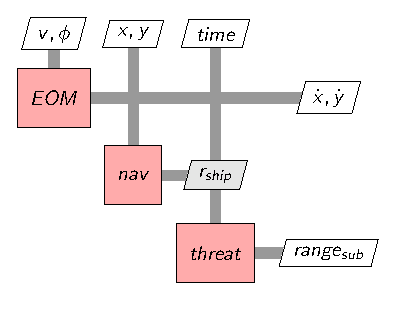
\includegraphics[scale=1.0]{images/donner_sub/donner_sub_ode_xdsm}
\end{frame}

\begin{frame}{The Donner Sub Problem: ODE}


    \lstset{basicstyle=\tiny}
    \lstinputlisting[language=Python]{../exercises/donner_sub/1_getting_started/donner_sub_ode.py}

    \pause
  
    \only<2>{
        \begin{tikzpicture}[overlay]
            \draw[red, very thick, ->] (8.5cm,3.75cm) to (7.1cm, 3.75cm);
        \end{tikzpicture}
  
        \begin{textblock*}{6cm}(9.75cm,4.7cm)
            \footnotesize \textcolor{red}{All ODE models accept num\_nodes}
        \end{textblock*}
  }
  
  \pause
  
    \only<3>{
        \begin{tikzpicture}[overlay]
            \draw[red, very thick, ->] (6.2cm,1.50cm) to (7.2cm, 1.50cm);
        \end{tikzpicture}

        \begin{textblock*}{7cm}(1.5cm,7.0cm)
            \footnotesize \textcolor{red}{Size ExecComp variables appropriately}
        \end{textblock*}
  }

\end{frame}     % Error is from the source code being outside the defined area (can ignore)


\begin{frame}{Setting up the problem}
    \begin{itemize}
      \item One phase (single ODE, no intermediate boundary constraints)
      \item Two state variables ($x$, $y$)
      \item One design parameter ($v$)
      \item One dynamic control ($\phi$)
      \item Objective: minimize $v$
    \end{itemize}
\end{frame}

\begin{frame}{Setting up the problem: Create the problem, trajectory, and phase}
    \lstset{basicstyle=\tiny}
    \lstinputlisting[language=Python,firstline=1,lastline=19]{../exercises/donner_sub/1_getting_started/exercise_1.py}
\end{frame}

\begin{frame}{What is a transcription, anyway?}
    \begin{itemize}
        \item Converts a continuous optimal control problem into a discrete NLP problem
        \item Key feature: The grid (or mesh), which controls the accuracy of the integration.
        \begin{itemize}
            \item More (or higher order) segments gives more accuracy at greater expense
        \end{itemize}
    \end{itemize}
\end{frame}

\begin{frame}{High-Order Legendre Gauss Lobatto Transcription}
    \begin{itemize}
        \item Developed by Herman and Conway
        \item Generalization of the older Hermite-Simpson method pioneered by Dickmanns and Wells and later Paris and Hargraves.
    \end{itemize}
\end{frame}

\begin{frame}{High-Order Legendre Gauss Lobatto Transcription}
    \animategraphics[loop,width=\textwidth]{3}{SourceCodes/dymos_animations/defect_convergence_lgl/frames/frame_}{00}{54}
\end{frame}

\begin{frame}{Radau Pseudospectral Method}
    \begin{itemize}
        \item Rao, Patterson, and Garg, et.al. at Univeristy of Florida.
        \item More variables than Gauss-Lobatto but only a single evaluation of the ODE per iteration.
    \end{itemize}
\end{frame}

\begin{frame}{Radau Pseudospectral Transcription}
    \animategraphics[loop,width=\textwidth]{3}{SourceCodes/dymos_animations/defect_convergence_lgr/frames/frame_}{00}{79}
\end{frame}

%
%\begin{frame}{Setting up the problem: Set options for the phase}
%    \lstset{basicstyle=\tiny}
%    \lstinputlisting[language=Python,firstline=19,lastline=33]{exercises/1_getting_started/exercise_1.py}
%\end{frame}
%
%
%\begin{frame}{Setting up the problem: Setup the driver and the recorder}
%    \lstset{basicstyle=\tiny}
%    \lstinputlisting[language=Python,firstline=33,lastline=50]{exercises/1_getting_started/exercise_1.py}
%\end{frame}
%
%
%\begin{frame}{Setting up the problem: Set the initial values and run the problem}
%    \lstset{basicstyle=\tiny}
%    \lstinputlisting[language=Python,firstline=52,lastline=65]{exercises/1_getting_started/exercise_1.py}
%\end{frame}
%
%
%\begin{frame}{Exercise 1: Solve the problem}
%    \centering
%    (This is really just a test to see if Dymos works on your system)
%\end{frame}
%
%\begin{frame}{Results of the first run}
%    \lstset{basicstyle=\tiny}
%    \lstinputlisting[firstline=127,lastline=128]{SourceCodes/donner_sub/1/SNOPT_print.out}
%\end{frame}
%
%\begin{frame}{What went wrong?}
%    \begin{block}{SNOPT\_print.out}
%        \lstset{basicstyle=\tiny}
%        \lstinputlisting[firstline=100,lastline=110]{SourceCodes/donner_sub/1/SNOPT_print.out}
%    \end{block}
%\end{frame}
%
%\begin{frame}{What went wrong?}
%    Our ship radius calculation is singular at the origin.
%    \centering
%    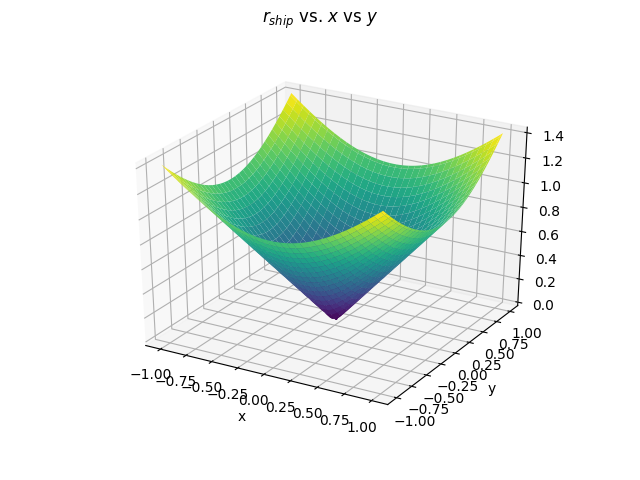
\includegraphics[scale=0.5]{images/donner_sub/ship_radius_plot.png}
%\end{frame}
%
%\begin{frame}{Avoiding the singularity}
%    \begin{columns}[T]
%    \column{0.5 \textwidth}
%        Change our path constraint function to this
%        \begin{align*}
%            r_{ship}^2 &= x^2 + y^2\\
%            r_{ship}^2 - time^2 &\ge 0
%        \end{align*}
%
%    \column{0.5 \textwidth}
%        \centering
%        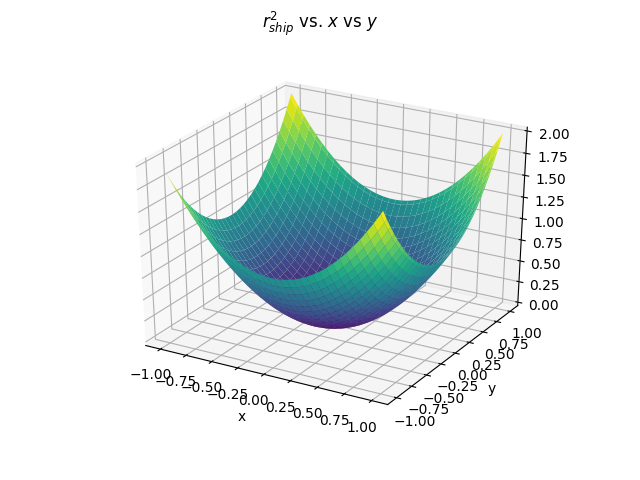
\includegraphics[scale=0.5]{images/donner_sub/ship_radius_plot2.png}
%    \end{columns}
%\end{frame}
%
%\begin{frame}{Exercise 2: Run the problem with a better constraint formulation}
%    \centering
%    Change the threat component to use
%    \begin{align*}
%        r_{ship}^2 - time^2 &\ge 0
%    \end{align*}
%\end{frame}
%
%\begin{frame}{Rerun the problem with this fix and...}
%    \begin{block}{SNOPT\_print.out}
%        \lstset{basicstyle=\tiny}
%        \lstinputlisting[firstline=129,lastline=131]{SourceCodes/donner_sub/2/SNOPT_print.out}
%    \end{block}
%\end{frame}
%
%\begin{frame}{Now what?}
%    From our initial guess
%    \begin{itemize}
%        \item The ship passes right through the sub origin.
%        \item The control history ($\phi$) is compatible with this solution.
%        \item Should the ship pass north or south?  Both have equal impact!
%        \item Our initial guess is a stationary point.
%    \end{itemize}
%\end{frame}
%
%\begin{frame}{Exercise 2 part 2: Change the initial guess to help the optimizer}
%    \begin{itemize}
%        \item Change the heading angle guess so it linearly changes from 80 deg to 100 deg.
%        \item This is enough to suggest a northern route around the sub.
%    \end{itemize}
%    \pause
%    \only<2> {
%        \lstinputlisting[language=Python,firstline=54,lastline=60,basicstyle=\tiny]{exercises/2_a_better_constraint/exercise_2_solution.py}
%    }
%\end{frame}
%
%\begin{frame}{Improving performance with coloring}
%    \begin{itemize}
%        \item Our current file will bog down if we increase the number/order of the segments (the curse of dimensionality)
%        \item Pseudospectral methods are particularly efficient when we can take advantage of the sparsity of the Jacobian matrix
%        \item Tell the driver to dynamically compute the coloring of our problem
%        \item OpenMDAO can do this regardless of your overall problem layout!
%    \end{itemize}
%\end{frame}
%
%\begin{frame}{Exercise 3: Tell the driver to use dynamic ``coloring'' to efficiently compute derivatives}
%    \pause
%    \only<2> {
%        \centering
%        \lstinputlisting[language=Python,firstline=46,lastline=46,basicstyle=\scriptsize]{exercises/3_coloring/exercise_3_solution.py}
%    }
%\end{frame}
%
%
%\begin{frame}{Lets look at the coloring pattern OpenMDAO found}
%    \lstinputlisting[language=Python,firstline=1,lastline=13,basicstyle=\tiny]{SourceCodes/donner_sub/4_coloring/output.txt}
%\end{frame}
%
%\begin{frame}{Graphically viewing the sparsity}
%    \begin{commandlineblock}{OpenMDAO command line utility}
%        \begin{verbatim}
%
%        \small
%        openmdao view\_coloring coloring\_files/total\_coloring.pkl -j
%
%        \end{verbatim}
%    \end{commandlineblock}
%\end{frame}
%
%\begin{frame}{Graphically viewing the sparsity}
%    \centering
%    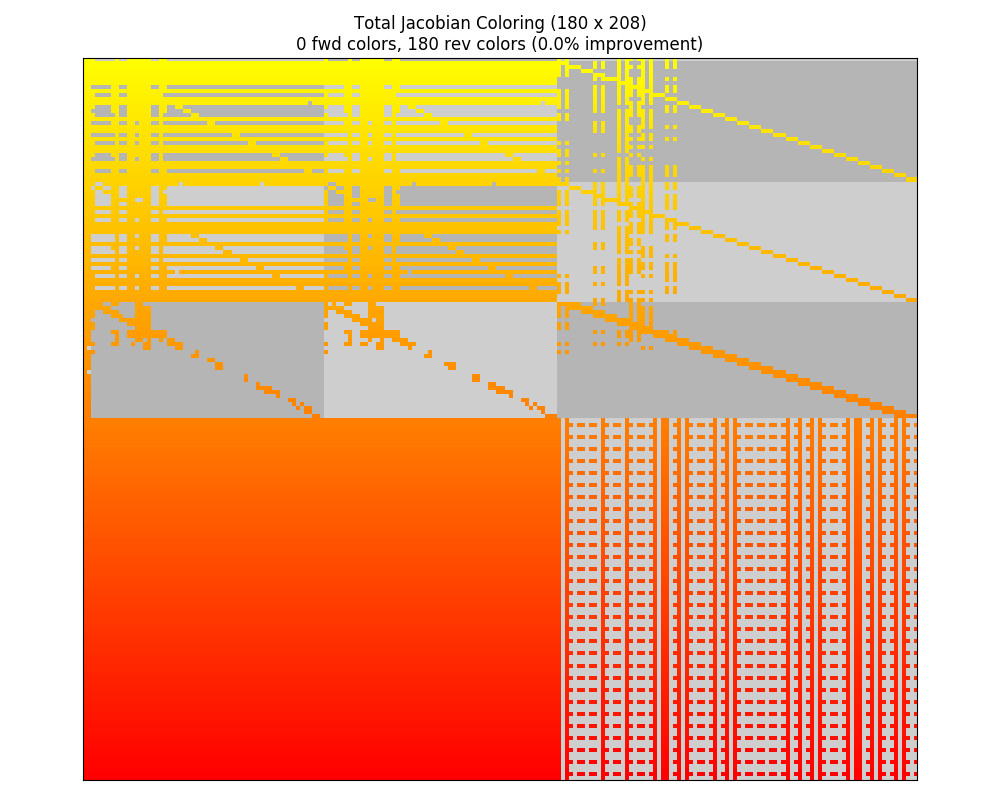
\includegraphics[scale=0.32]{images/donner_sub/total_jacobian_coloring.png}
%
%    \pause
%
%    \only<2>{
%        \begin{tikzpicture}[overlay]
%            \draw[red, very thick, ->] (-5.5cm,3.75cm) to (-3.5cm, 2.75cm);
%        \end{tikzpicture}
%
%        \begin{textblock*}{4cm}(0.5,4.7cm)
%            \footnotesize \textcolor{red}{Our path constraint has a dense Jacobian!}
%        \end{textblock*}
%  }
%\end{frame}
%
%\begin{frame}{ExecComp does not provide sparse partials by default}
%    \begin{itemize}
%        \item Our ExecComp is providing a full $n$ x $n$ Jacobian
%        \item Use the \emph{has\_diag\_partials} option to tell ExecComp to provide a sparse diagonal of partials.
%    \end{itemize}
%    \centering
%\end{frame}
%
%\begin{frame}{Exercise 4: Fix the sparisty issue in the ODE}
%    \pause
%    \only<2> {
%    \centering
%    \lstinputlisting[language=Python,firstline=20,lastline=24,basicstyle=\scriptsize]{exercises/4_fixing_the_sparsity/donner_sub_ode_solution.py}
%    }
%\end{frame}
%
%\begin{frame}{Graphically viewing the sparsity}
%    \centering
%    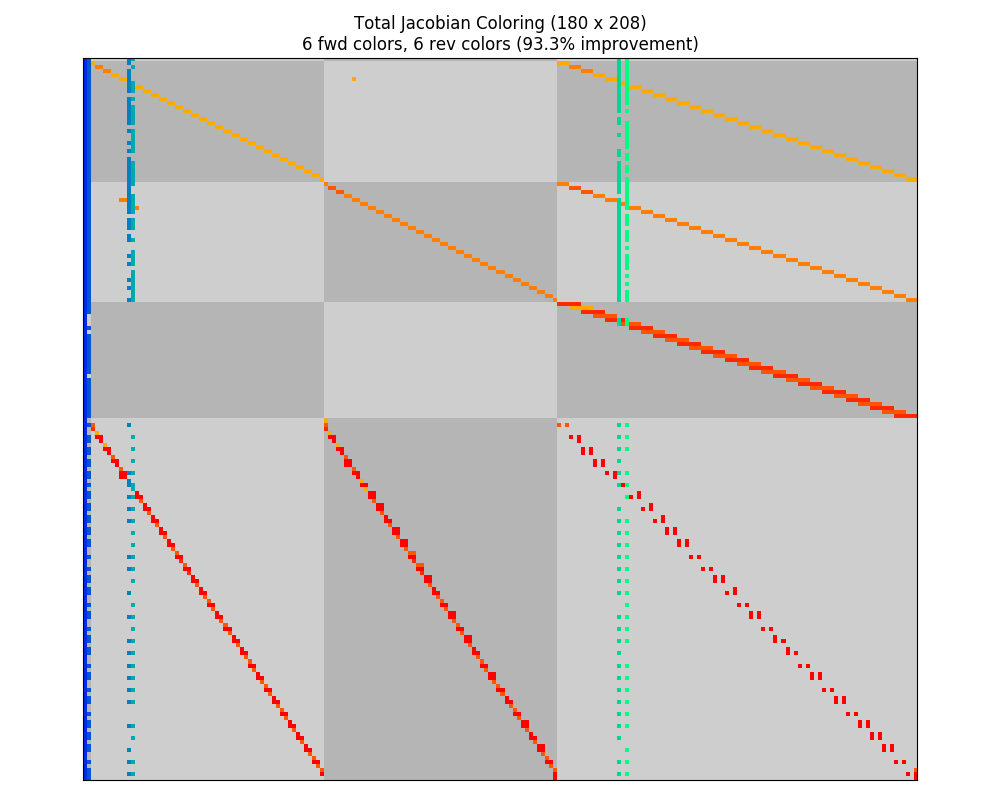
\includegraphics[scale=0.26]{images/donner_sub/total_jacobian_coloring2.png}
%
%    Runtime decreased from ~6 seconds to ~1 second!
%\end{frame}
%
%\begin{frame}{Is the solution accurate?}
%    \begin{itemize}
%        \item A converged solution is great, but meaningless if transcription cannot accurately represent the dynamics
%        \item We can simulate the trajectory with a variable step integrator (scipy.solve\_ivp) and see if we get the same solution.
%        \item We can simulate trajectory objects or phase objects with the simulate method
%        \begin{itemize}
%            \item Returns a problem instance with the same timeseries outputs as phase objects
%            \item Can optionally save the simulation problem to a recorded file
%        \end{itemize}
%    \end{itemize}
%\end{frame}
%
%\begin{frame}{Exercise 5: Perform explicit simulation of the solution}
%    \begin{itemize}
%        \item Call simulate after our solution is obtained to get an explicitly integrated result.
%        \item Save the result to ``donner\_sub\_simulation.sql''
%    \end{itemize}
%    \pause
%    \only<2> {
%    \lstinputlisting[language=Python,firstline=70,lastline=73,basicstyle=\scriptsize]{exercises/5_simulation/exercise_5_solution.py}
%    }
%\end{frame}
%
%\begin{frame}{Retrieving Results: Timeseries outputs}
%    \begin{itemize}
%        \item The phase timeseries component provides consistent output for all ODE variables of interest.
%        \item By default it captures the values of time, states, controls, design/input/trajectory parameters at all nodes in the phase.
%        \item Additional ODE output variables can be added through the add\_timeseries\_output method on Phase.
%    \end{itemize}
%\end{frame}
%
%\begin{frame}{Exercise 6: Store necessary results in the timeseries output}
%    \begin{itemize}
%        \item Add timeseries outputs for \emph{sub_range} and \emph{r_ship2}
%        \item Run \emph{plot_donner_sub_results.py}
%    \end{itemize}
%\end{frame}
%
%\begin{frame}{Plotting our results}
%    \lstinputlisting[language=Python,basicstyle=\scriptsize]{exercises/6_plotting_results/plot_donner_sub_results.py}
%\end{frame}
%
%\begin{frame}{Plotting our results}
%    \centering
%    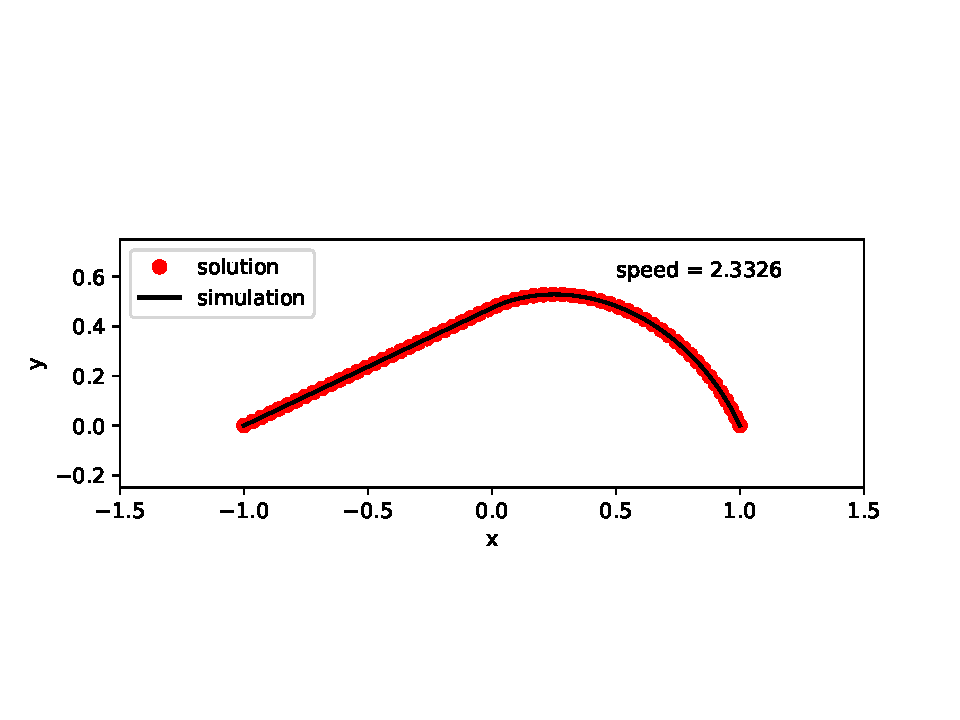
\includegraphics[scale=0.50]{exercises/6_plotting_results/solution_vs_simulation.pdf}
%\end{frame}
%
%\begin{frame}{Plotting our results}
%    \centering
%    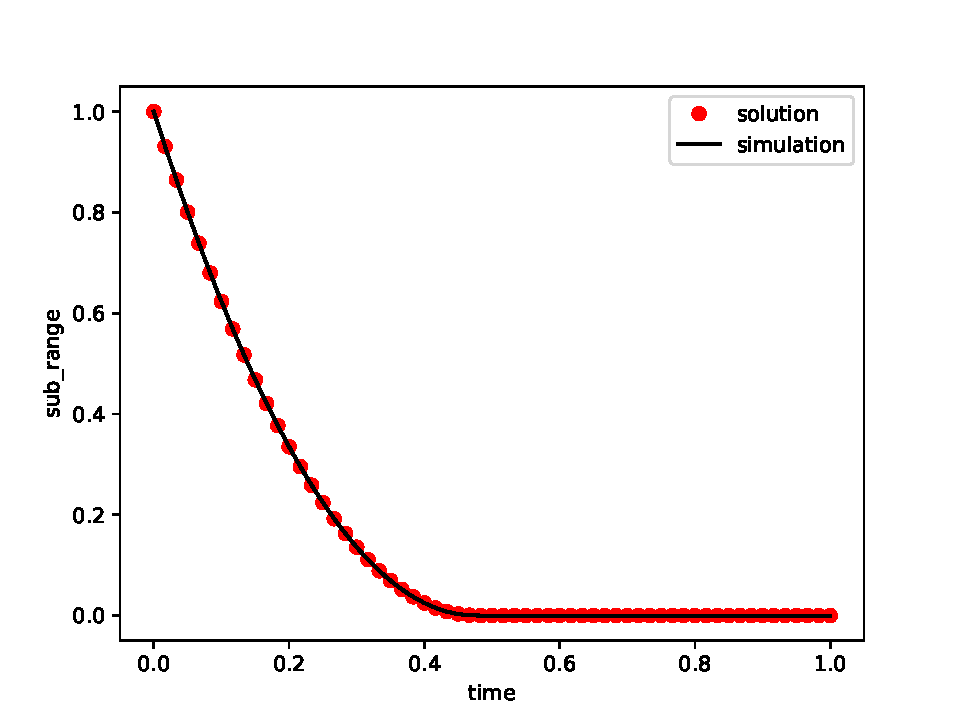
\includegraphics[scale=0.50]{exercises/6_plotting_results/sub_range_vs_time.pdf}
%\end{frame}
%
%\begin{frame}{Fixing inaccurate solutions}
%    \begin{itemize}
%        \item Solutions with insufficient grids \emph{typically} exhibit divergence of the solution and simulated trajectories.
%        \item We are currently implementing a grid refinement algorithm to automatically update the grid.
%        \this Capability is accessed via Dymos' \texttt{run\_problem} function.
%        \begin{itemize}
%            \item Dymos will search for all phases in a problem, and optionally refine each
%            \item Refinement options can be set on a phase-by-phase basis.
%        \end{itemize}
%    \end{itemize}
%\end{frame}
%
%\begin{frame}{Exercise 7: Refining the grid}
%    \begin{itemize}
%        \item Use the Dymos run_problem function to iteratively run the driver while refining the grid.
%    \end{itemize}
%    \pause
%    \only<2> {
%    \lstinputlisting[language=Python,basicstyle=\scriptsize,firstline=68,lastline=72]{exercises/7_grid_refinement/exercise_7_solution.py}
%    }
%\end{frame}
%
%\begin{frame}{The grid refinement summary}
%    \lstinputlisting[basicstyle=\tiny]{exercises/7_grid_refinement/grid_refinement.out}
%\end{frame}
%
%\begin{frame}{Using multiple phases to capture extremal values}
%    \begin{block}{What is the maximum/minimum value of y in this problem?}
%    \begin{itemize}
%        \item Path constraints only assess values at nodes
%        \item If we want to capture the true extremal value, how do we do that?
%        \begin{itemize}
%            \item Boundary constraints!
%            \item End the first phase at $\frac{dy}{dt} = 0$
%        \end{itemize}
%    \end{itemize}
%    \end{block}
%\end{frame}
%
%\begin{frame}{}
%    \begin{block}{Exercise 9}
%        \begin{itemize}
%            \item Add a second phase to the problem
%            \item Link time, states, and controls of the phases for continuity
%            \item Modify boundary constraints as necessary
%            \item Add speed as a trajectory design parameter
%    \end{block}
%\end{frame}


\end{document}
